
Para a apresentação dos resultados, é de interesse citar novamente os objetivos estabelecidos no Capítulo \ref{def_problem}. Desejávamos integrar a biblioteca OpenVDB ao Blender, de modo a permitir a visualização de volumes e dados tridimensionais salvos em arquivos desta biblioteca. No entanto, o módulo do software responsável pelos cálculos de iluminação para a exibição do resultado final está em desenvolvimento por outros desenvolvedores e ainda não é funcional.

Por isso, um artifício será utilizado na exibição dos resultados. A consulta aos valores armazenados na textura, ou seja, a amostragem dos pontos será avaliada por fatias, que, neste caso, serão planos, posicionados próximos uns aos outros, de modo a dar a impressão de visualizarmos um volume. A visualização de valores interiores ao volume será dada pelo uso de apenas um plano. Esta estratégia de visualização é exibida na Figura \ref{render_approach}.

%figura aqui!! :-P
\begin{figure}[!htb]
\center
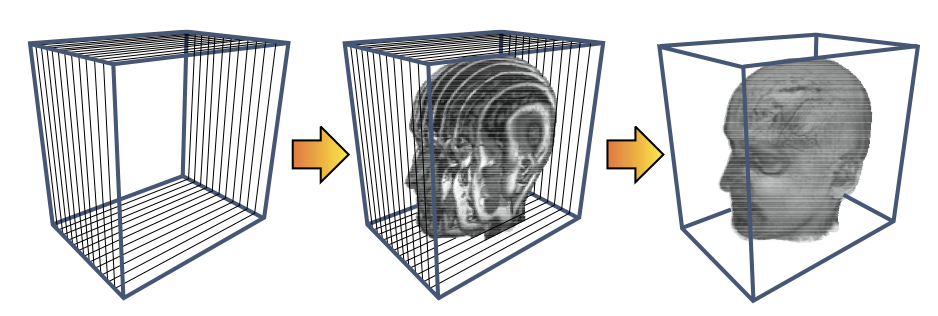
\includegraphics[width=13cm]{2drendering_approach}
\caption{À esquerda, a geometria que conterá os pontos amostrados: uma pilha de planos. No centro, a avaliação dos dados volumétricos em cada uma das fatias. À direita, o resultado da renderização, dando a impressão de visualização de um volume.}
\label{render_approach}
\end{figure}

O volume utilizado para exemplificar o funcionamento da biblioteca no Blender é exibido na Figura \ref{fig:vdb_view1}, e um corte transversal, para visualizarmos seus dados internos, é exibido nas Figuras \ref{fig:vdb_view2} e \ref{fig:vdb_view3}.

\begin{figure}[H]
        \centering
        \begin{subfigure}{0.3\textwidth}
                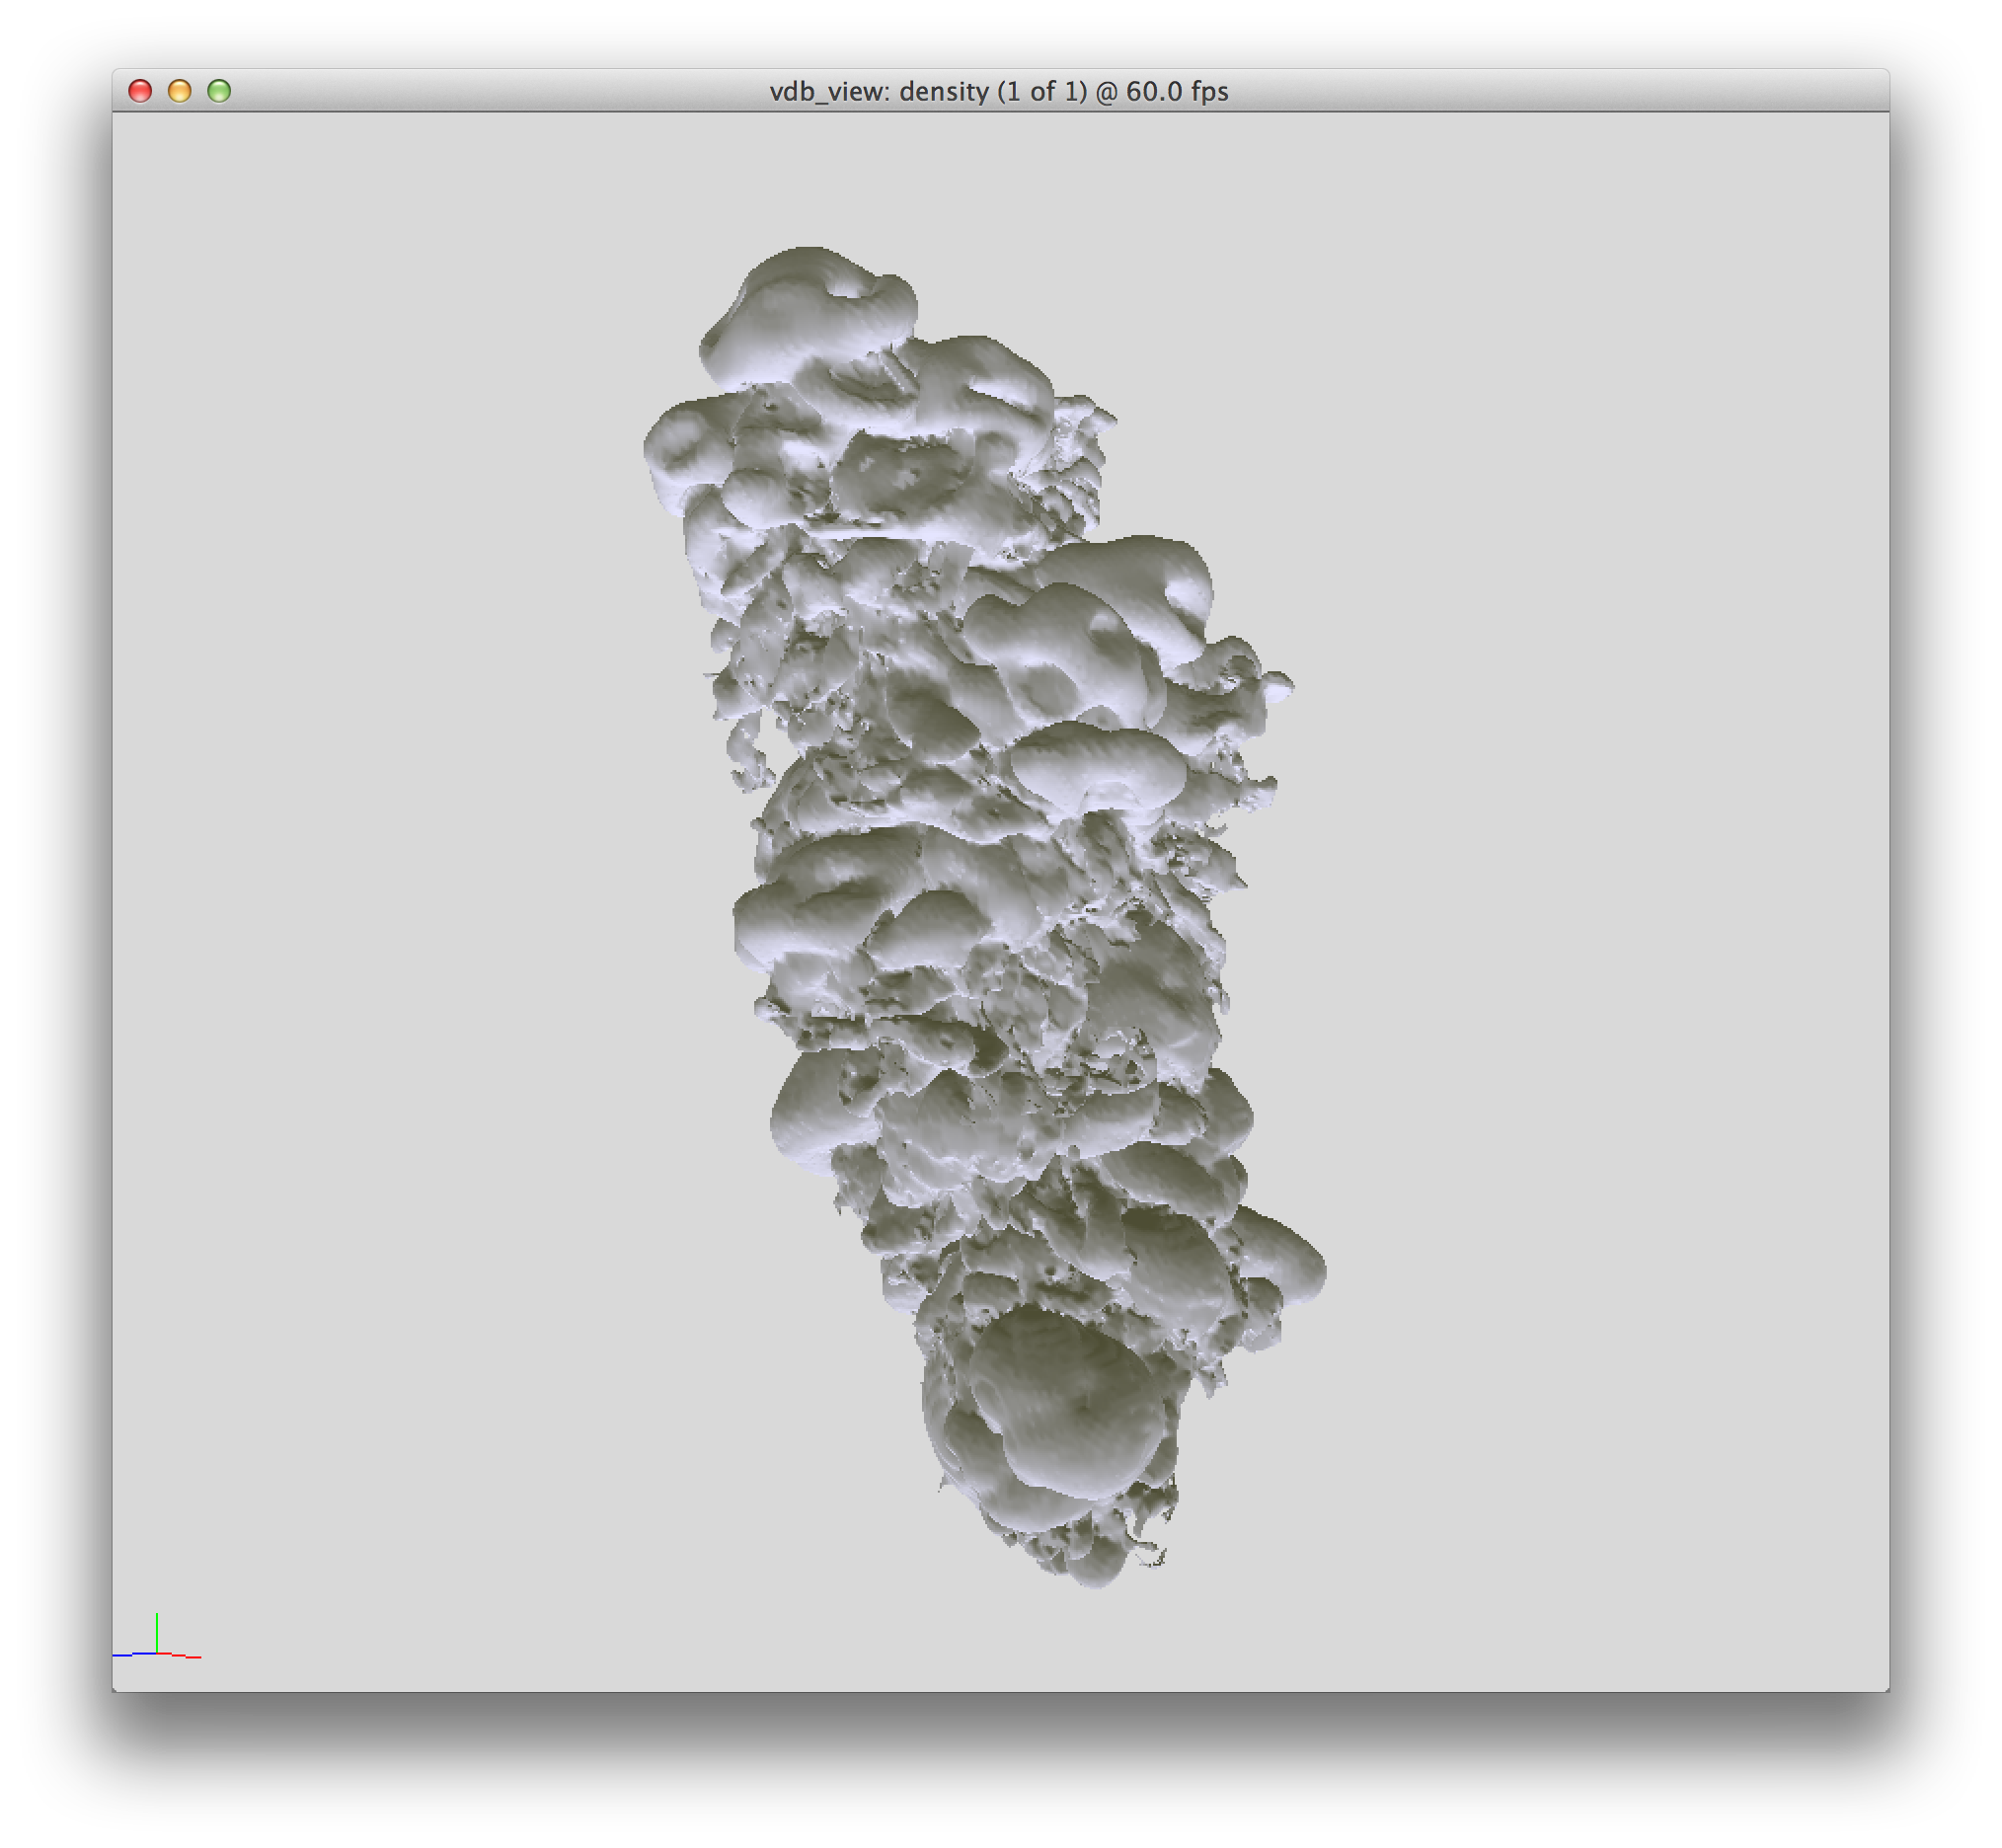
\includegraphics[width=\textwidth]{vdb_view1}
                \caption{Visão externa.}
                \label{fig:vdb_view1}
        \end{subfigure}%
        ~ %add desired spacing between images, e. g. ~, \quad, \qquad etc.
          %(or a blank line to force the subfigure onto a new line)
        \begin{subfigure}{0.3\textwidth}
                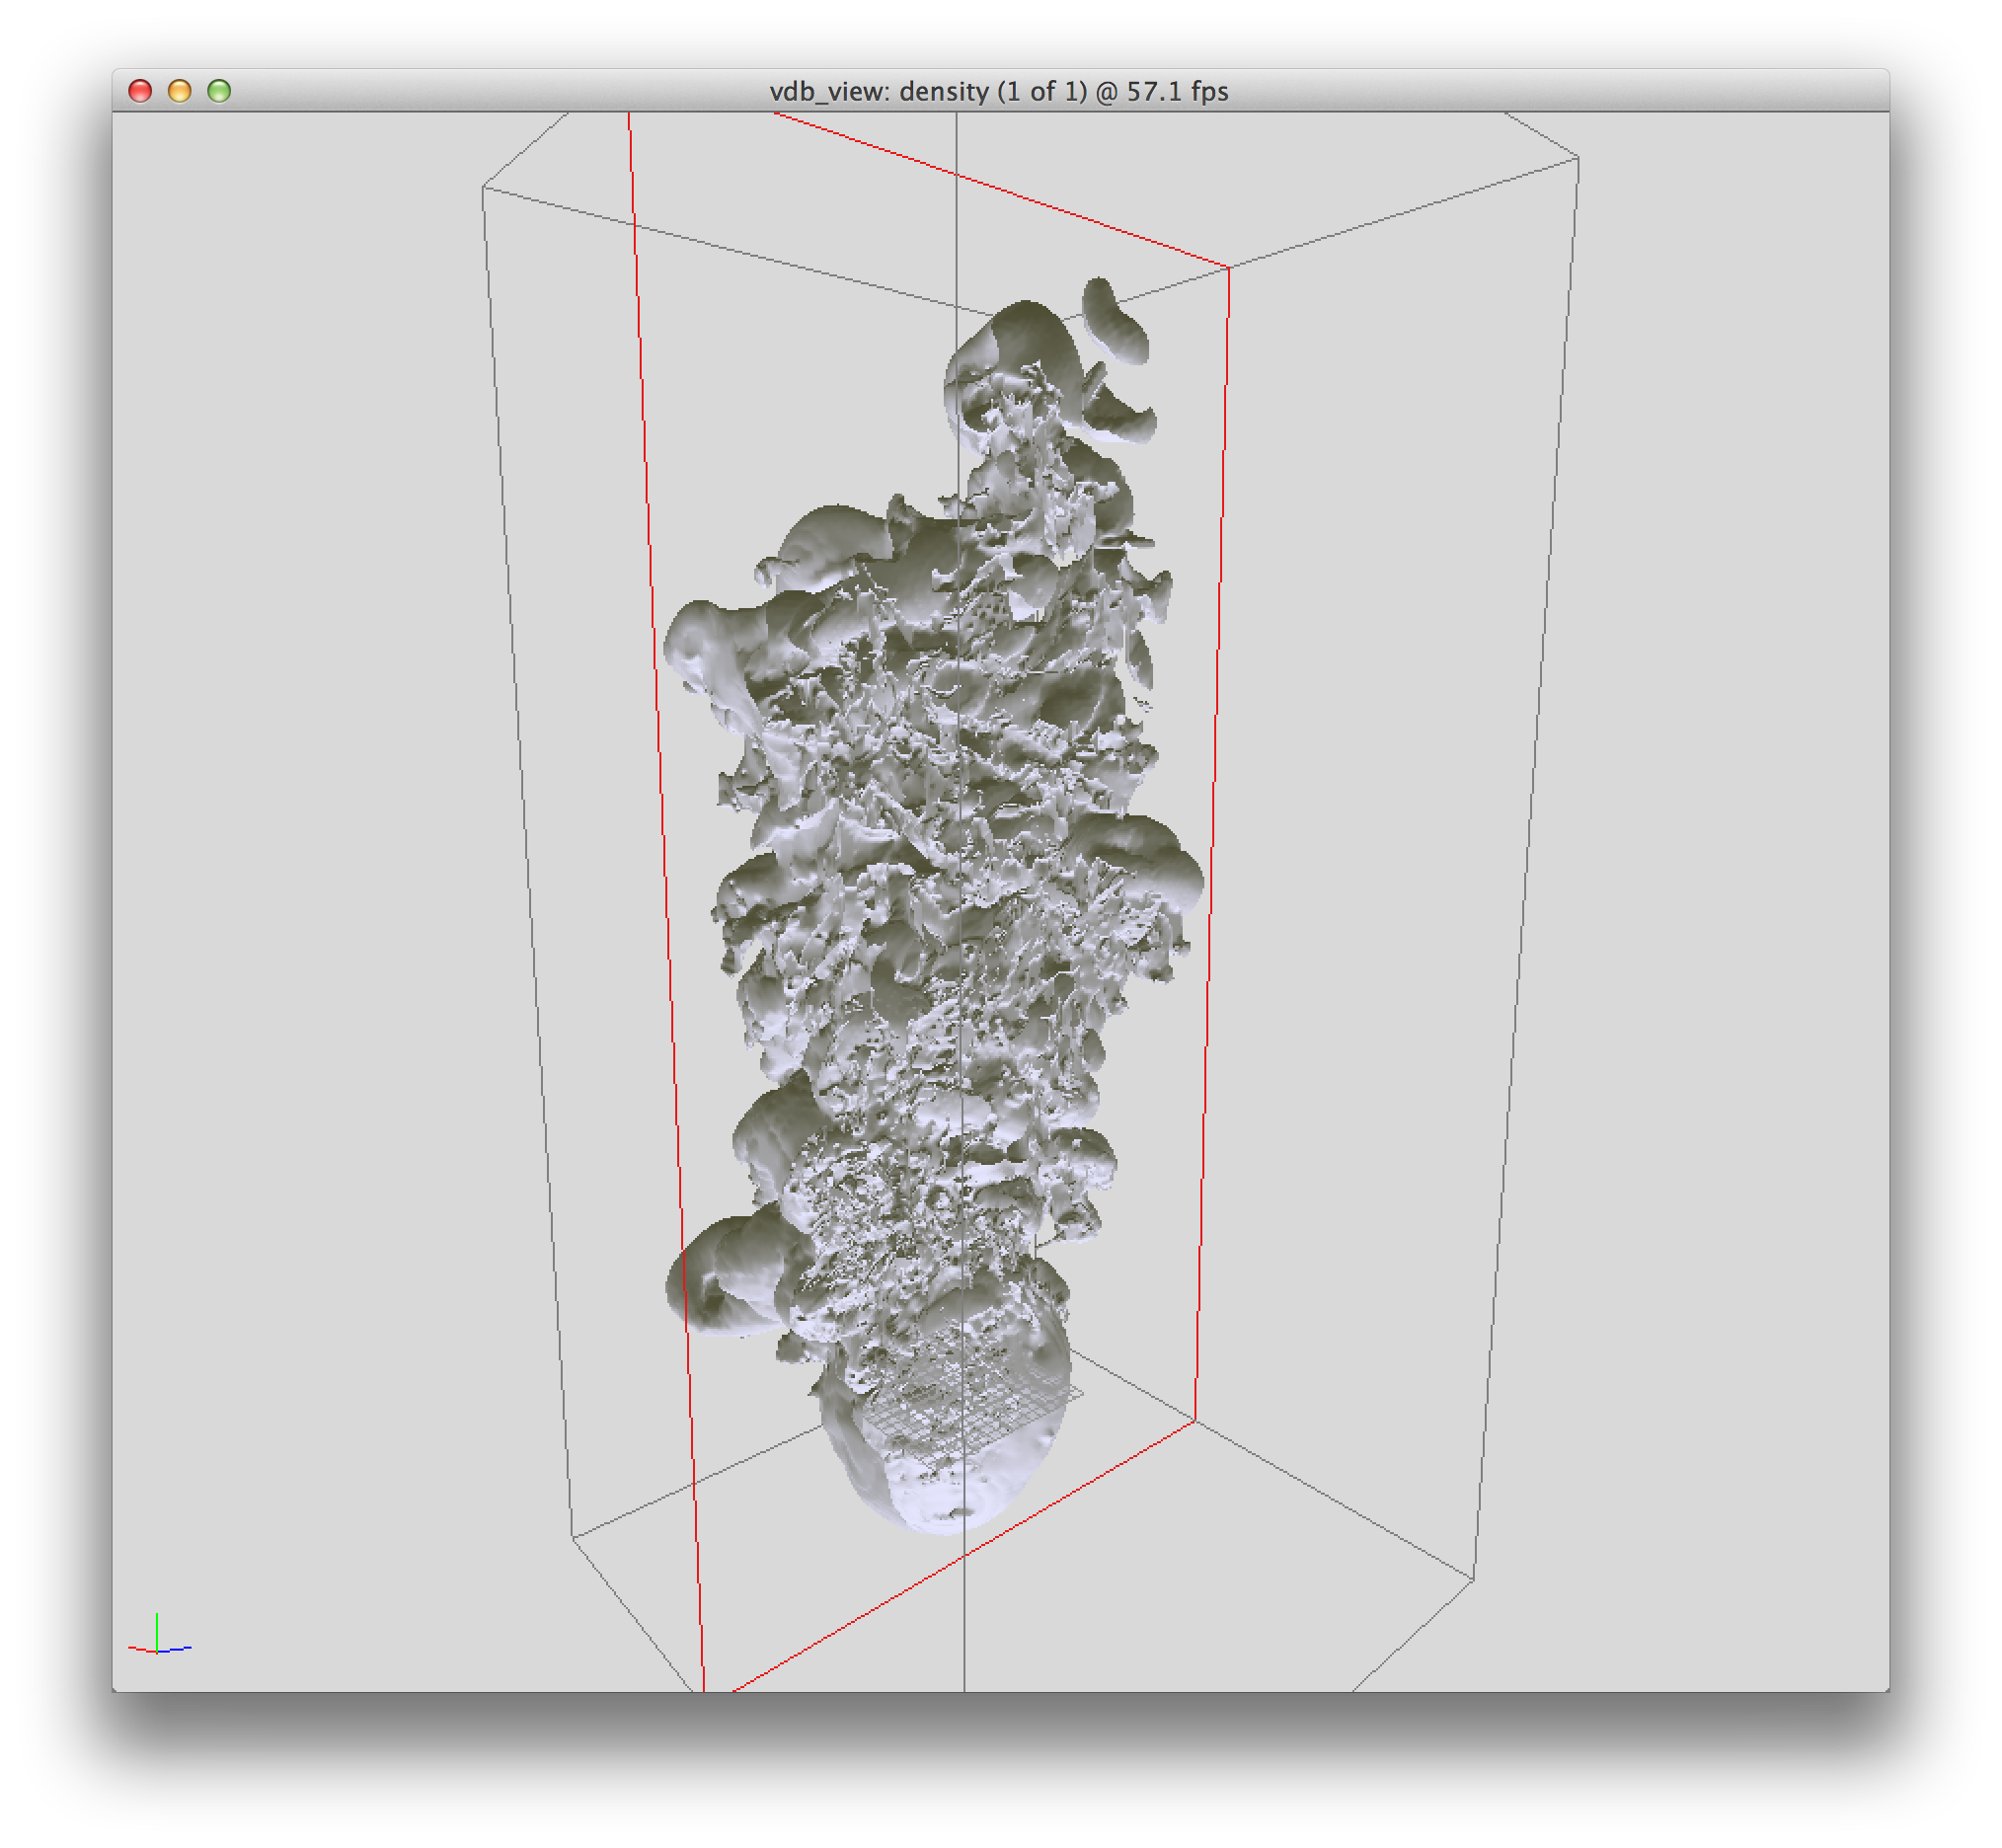
\includegraphics[width=\textwidth]{vdb_view2}
                \caption{Visão interna.}
                \label{fig:vdb_view2}
        \end{subfigure}
        ~ %add desired spacing between images, e. g. ~, \quad, \qquad etc.
          %(or a blank line to force the subfigure onto a new line)
        \begin{subfigure}{0.3\textwidth}
                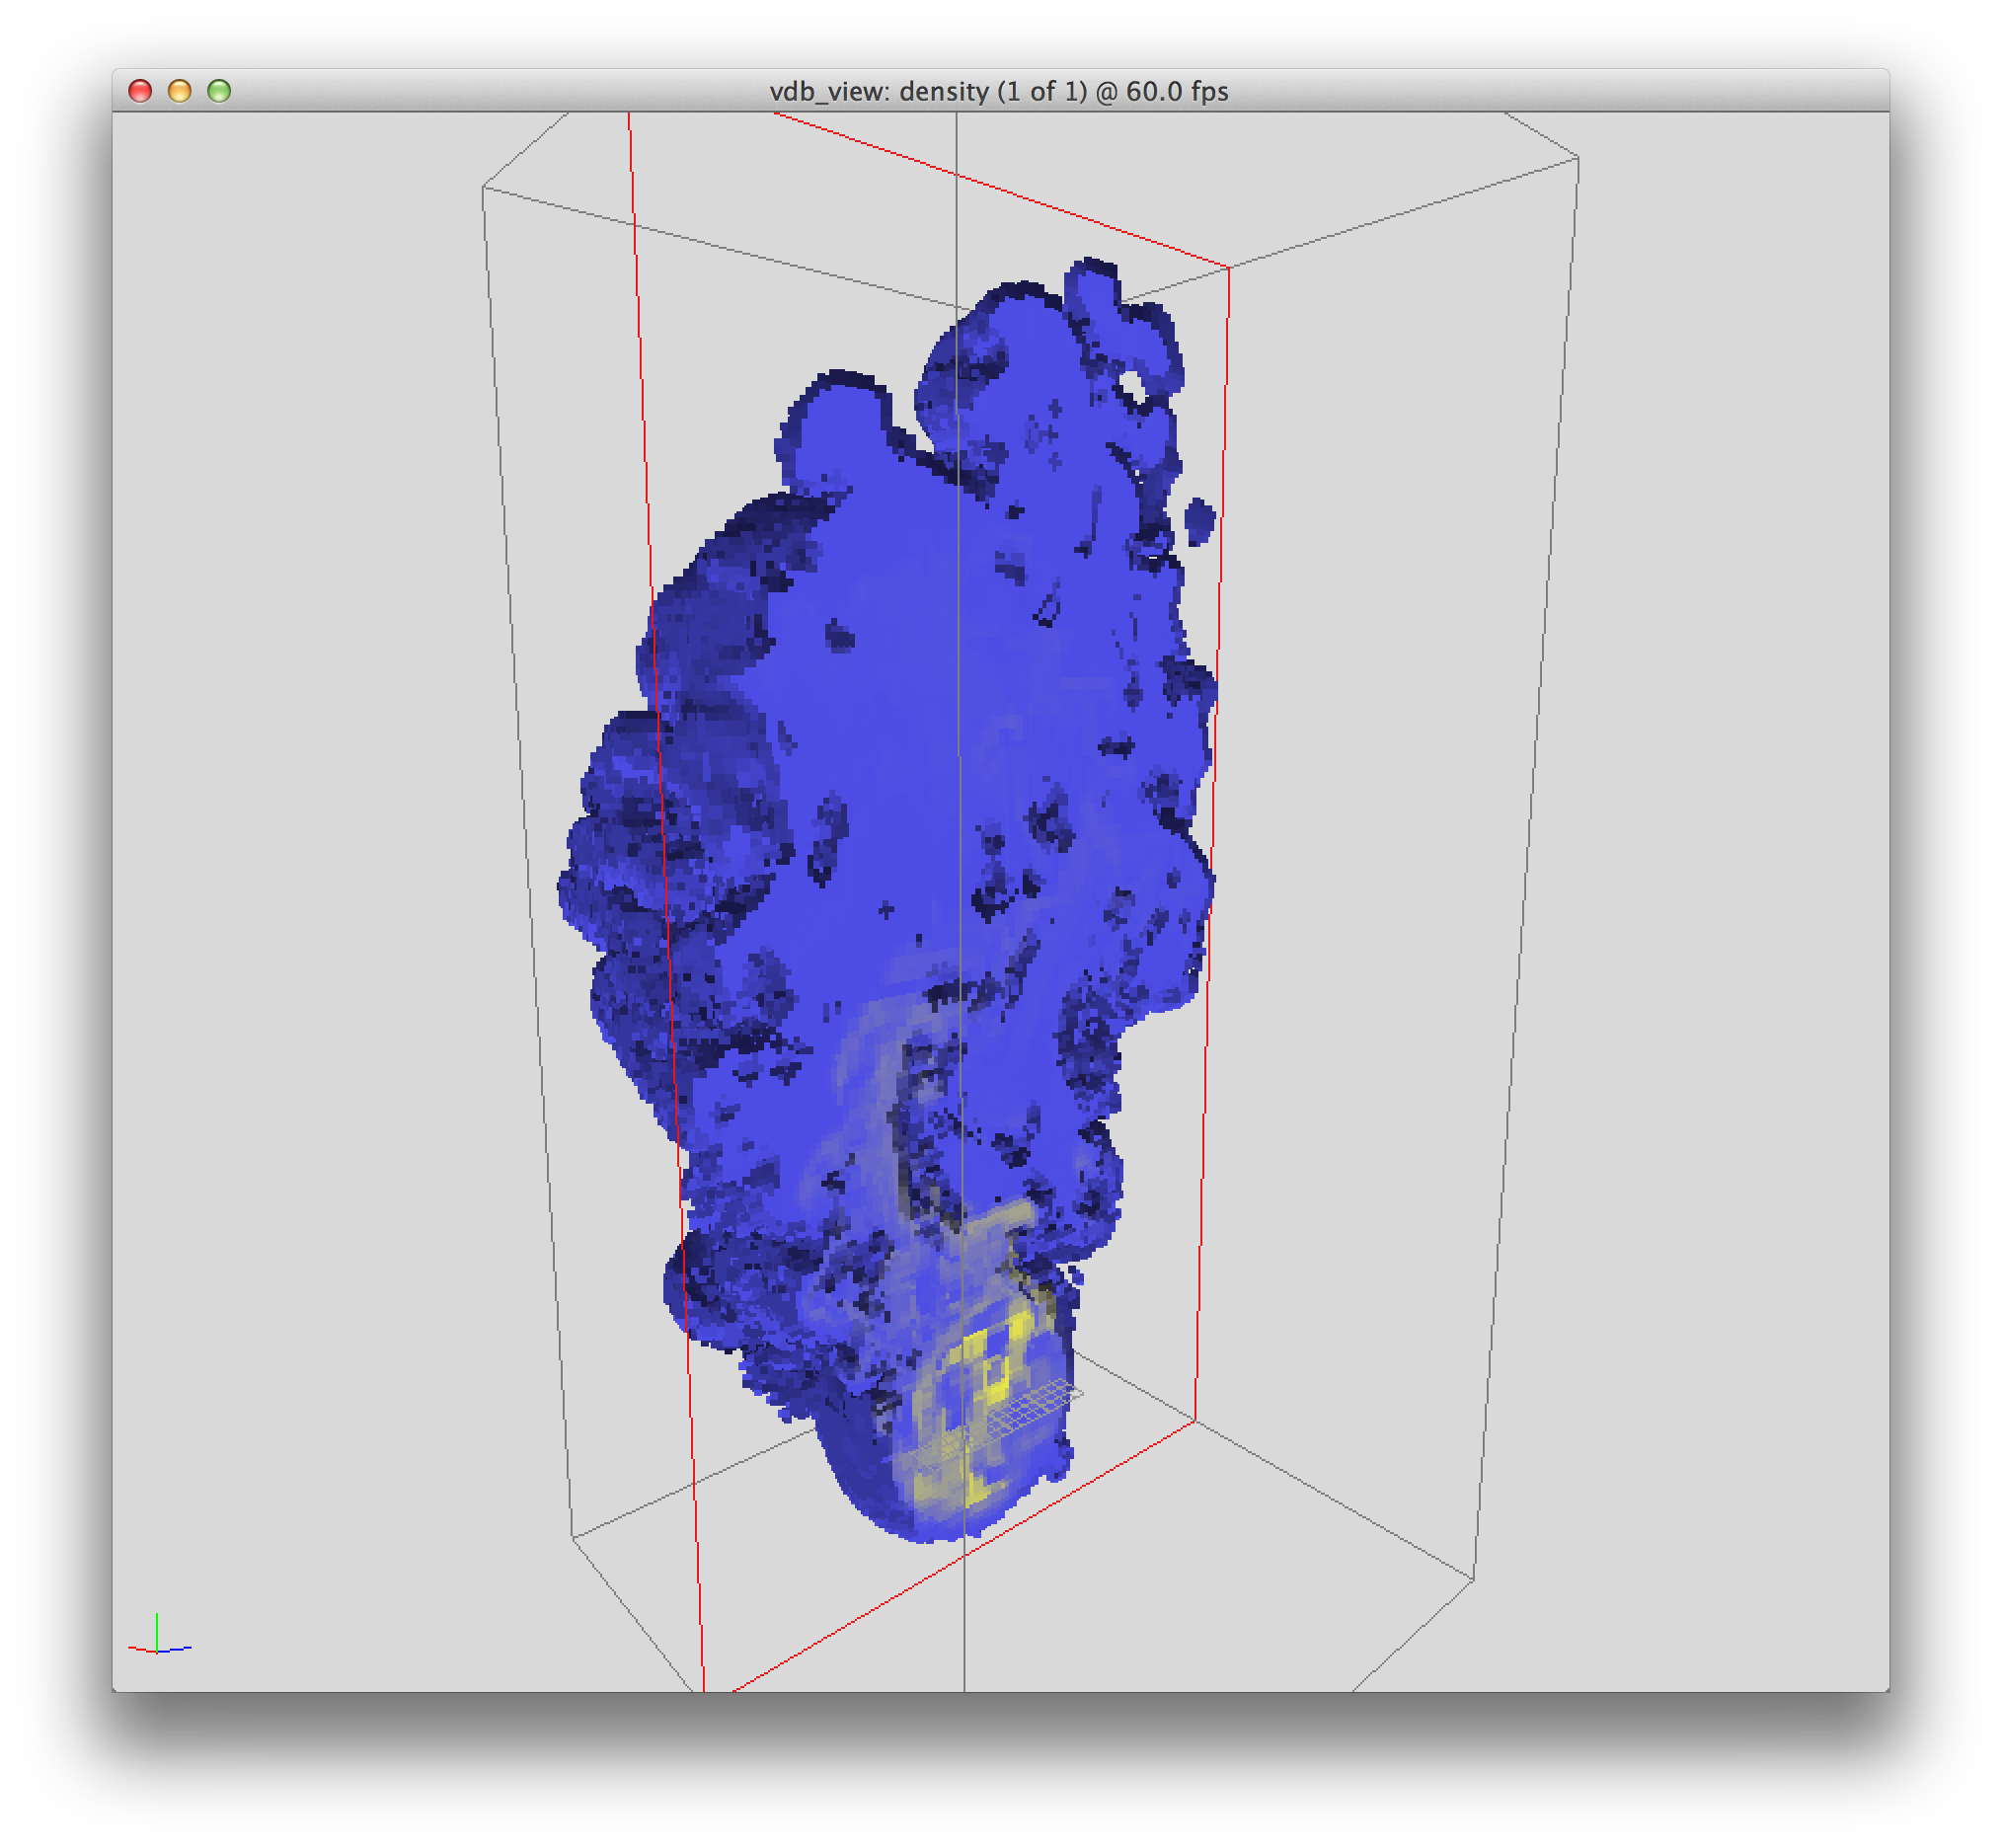
\includegraphics[width=\textwidth]{vdb_view3}
                \caption{Valores, por cor.}
                \label{fig:vdb_view3}
        \end{subfigure}
        \caption{Volume representando a densidade de uma fumaça, usada no exemplo apresentado, exibido por um visualizador específico para o formato VDB.}\label{fig:vdb_view}
\end{figure}


No Blender, o arquivo de exemplo, \texttt{smoke.vdb}, é carregado através de um nó implementado em Open Shading Language, exibido na Figura \ref{vdb_node}. E na Figura \ref{vdb_blender_interface}, a interface do Blender com a pré-visualização do mesmo volume mostrado na Figura \ref{fig:vdb_view} é exibido. As cores de exibição, que estão diferentes entre as representações, é facilmente configurável no Blender, se desejado.
\iffalse
	Opening file: /Users/rafael/Documents/vdb_files/smoke.vdb
VDB file loaded. Volume details: 

creator: Houdini/SOP_OpenVDB_Write
Grid name: density
Grid value type: float
 class: fog volume
 file_bbox_max: [111, 223, 112]
 file_bbox_min: [1, 2, 1]
 file_mem_bytes: 6.984.656
 				10.793.640
 file_voxel_count: 1049275
 is_local_space: false
 is_saved_as_half_float: true
 name: density
 roiMax: [112, 224, 113]
 roiMin: [0, 0, 0]
 value_type: float
 vector_type: invariant
\fi
%figura aqui!! :-P
\begin{figure}[!htb]
\center
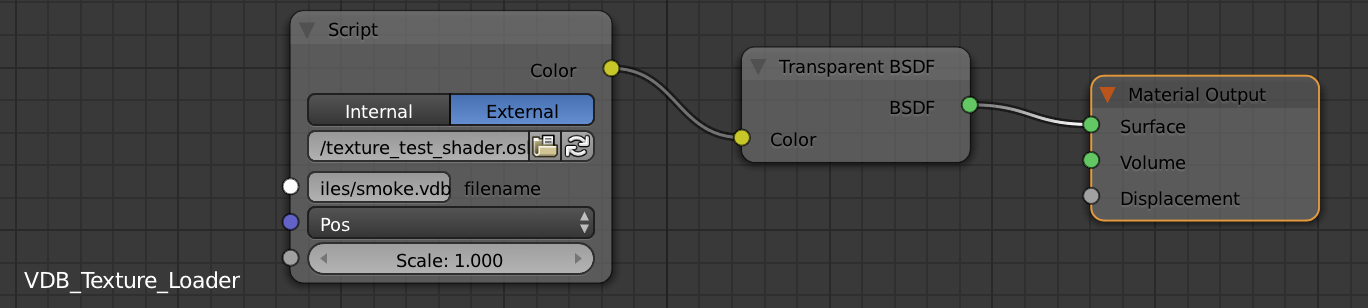
\includegraphics[width=12cm]{vdb_node}
\caption{Nó gerado a partir de código OSL especificamente para carregar arquivos VDB.}
\label{vdb_node}
\end{figure}

%figura aqui!! :-P
\begin{figure}[!htb]
\center
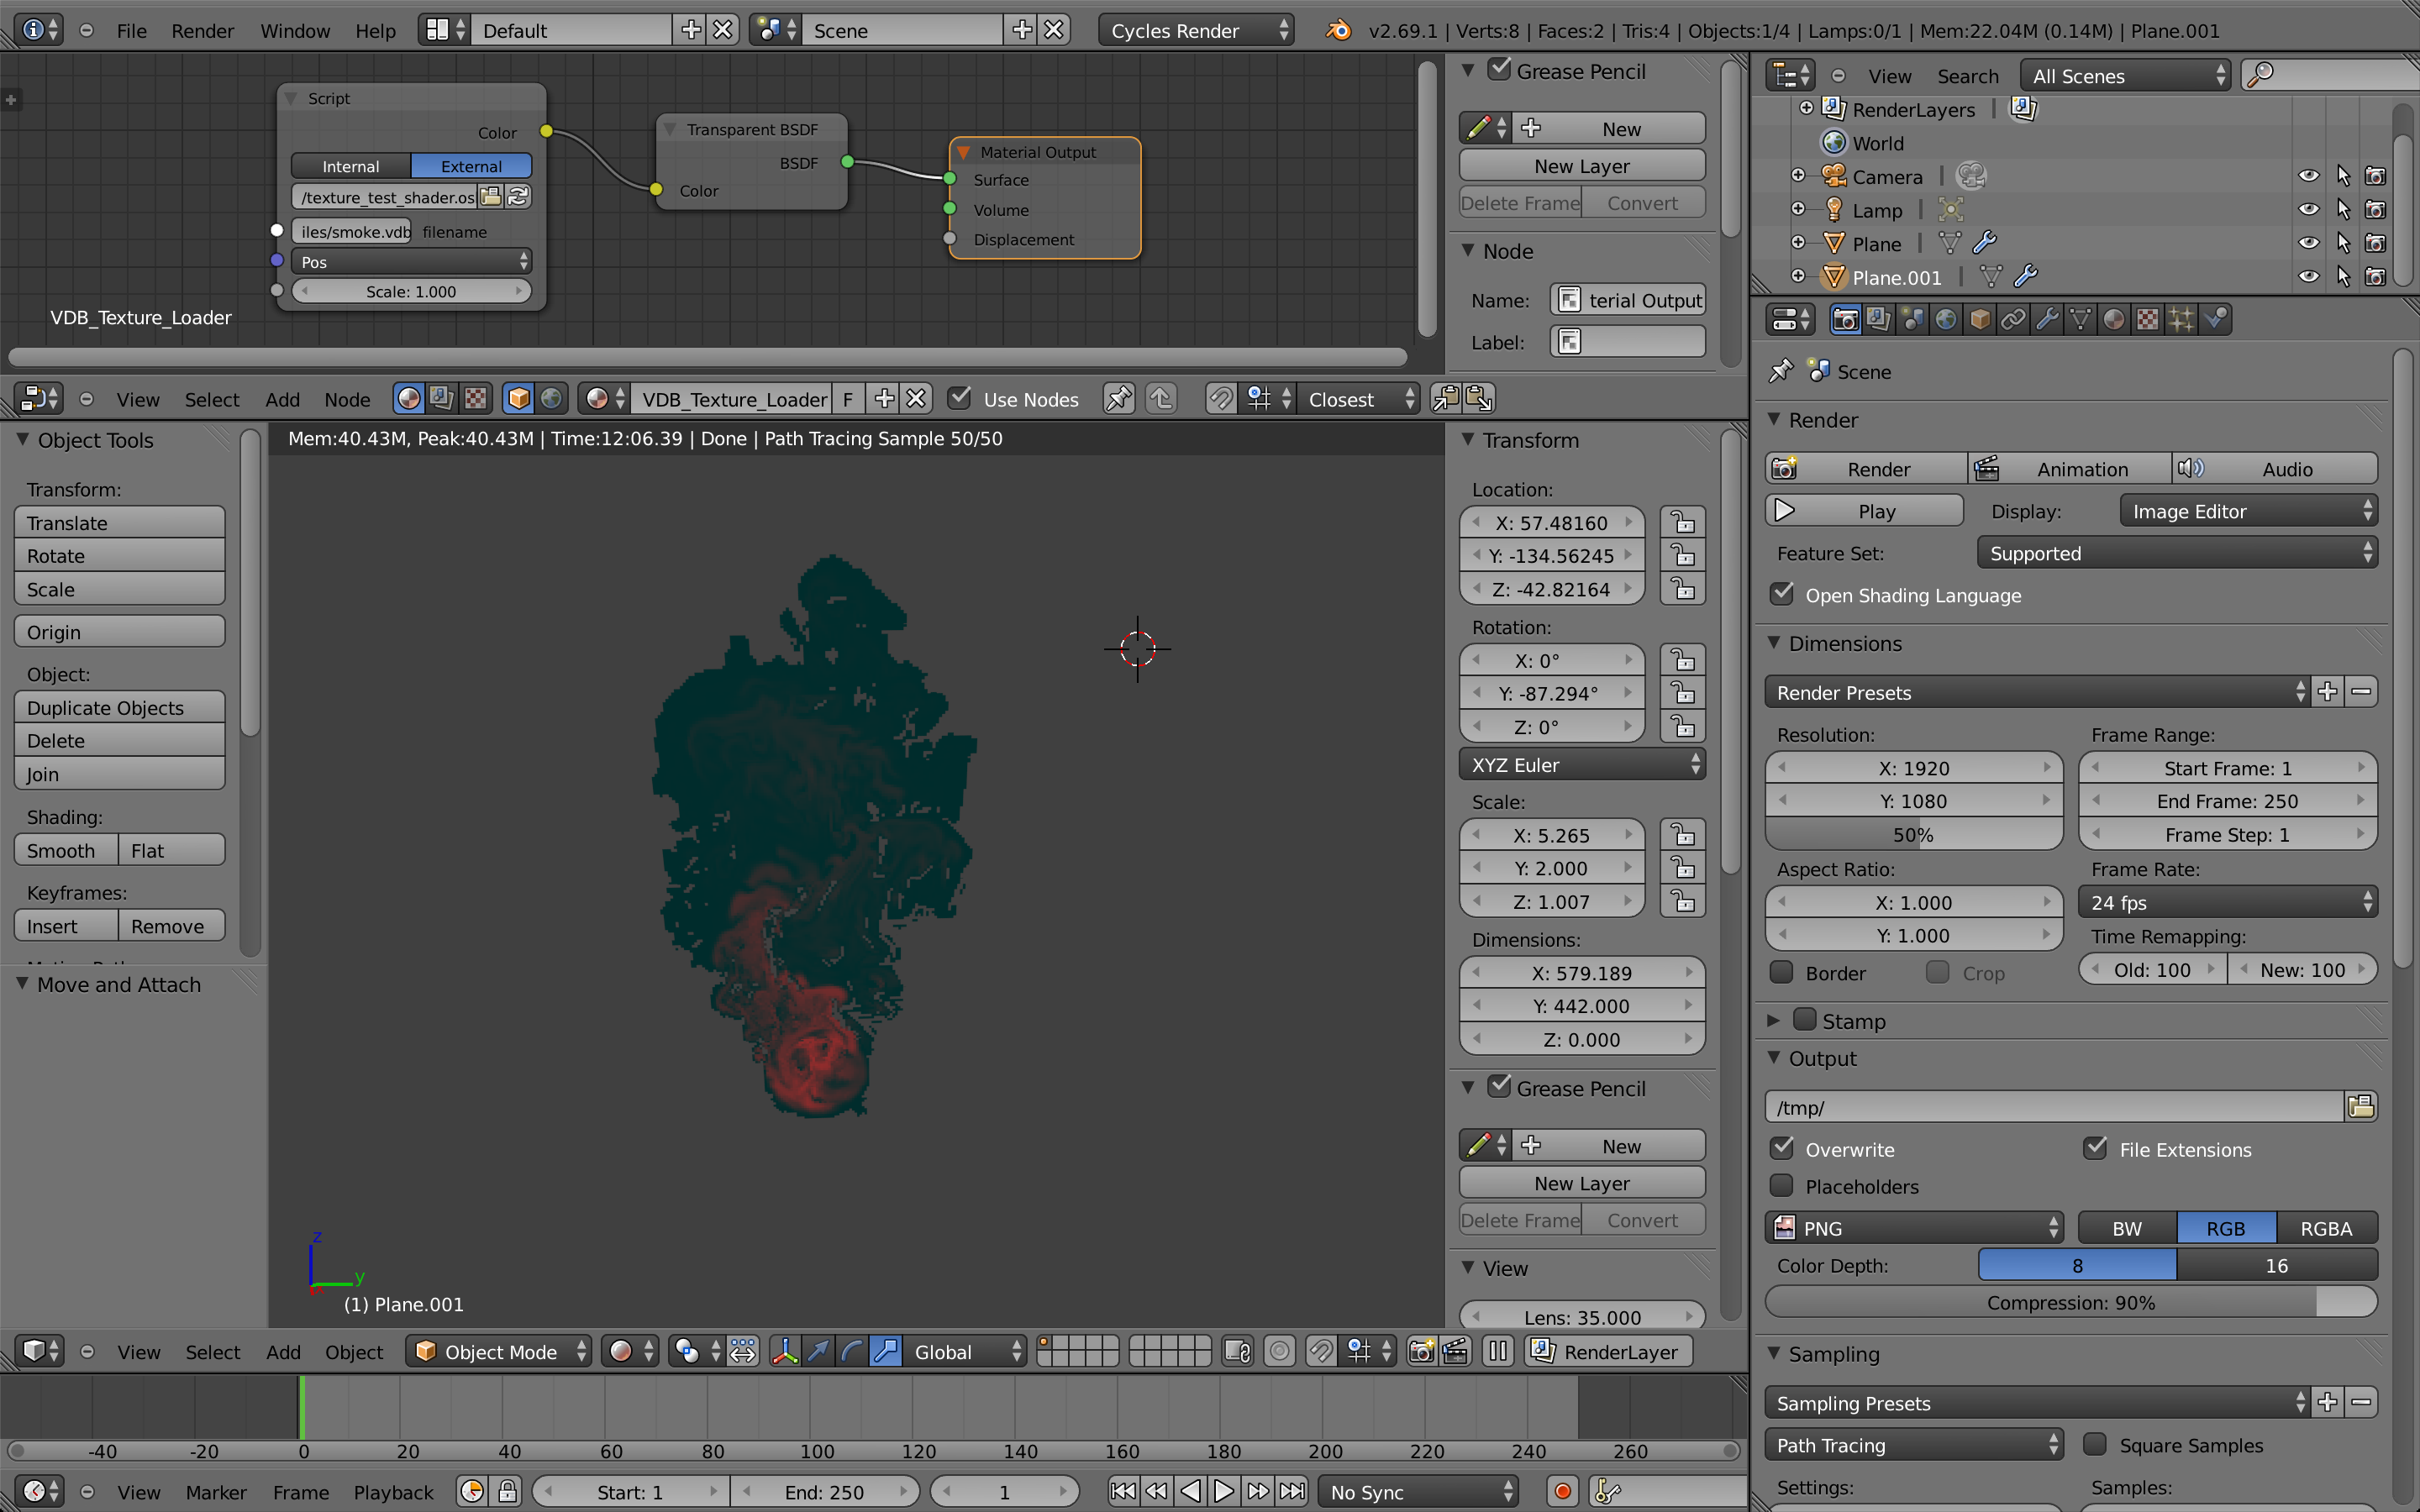
\includegraphics[width=12cm]{vdb_blender_interface}
\caption{Interface do Blender com a pré-visualização de uma fatia do volume.}
\label{vdb_blender_interface}
\end{figure}